\RequirePackage[2020-02-02]{latexrelease}


% Template for seminar reports
% Computer Vision Group, Visual Computing Institute, RWTH Aachen University
\documentclass[twoside,a4paper,article]{combine}
\usepackage[utf8]{inputenc}
\usepackage{a4}
\usepackage{fancyhdr}   
%\usepackage{german}    % Uncomment this iff you're writing the report in German
\usepackage{makeidx}
\usepackage{color}
\usepackage{t1enc}		% German letters in the "\hyphenation" - command
\usepackage{latexsym}	% math symbols
\usepackage{amssymb}    % AMS symbol fonts for LaTeX.
\usepackage{graphicx}
\usepackage{pslatex}
\usepackage{ifthen}
\usepackage{booktabs}
\usepackage[T1]{fontenc}
\usepackage{pslatex}
\usepackage{psfrag}
\usepackage{subfigure}
\usepackage{url}
\usepackage{datetime}
\usepackage{xspace}
\usepackage{newtxmath}

\usepackage{float}
\usepackage{subcaption}

\usepackage[table]{xcolor}% http://ctan.org/pkg/xcolor
\usepackage{listings}



\newdateformat{monthyeardate}{\monthname[\THEMONTH] \THEYEAR}

% Do not change these sizes and do not add superfluous 
% pagebreaks to increase the page count.
\setlength{\oddsidemargin}{3.6pt}
\setlength{\evensidemargin}{22.6pt}
\setlength{\textwidth}{426.8pt}
\setlength{\textheight}{654.4pt}
\setlength{\headsep}{18pt}
\setlength{\headheight}{15pt}
\setlength{\topmargin}{-41.7pt}
\setlength{\topskip}{10pt}
\setlength{\footskip}{42pt}
\setlength{\parindent}{0pt}

\makeatletter
\DeclareRobustCommand\onedot{\futurelet\@let@token\@onedot}
\def\@onedot{\ifx\@let@token.\else.\null\fi\xspace}
\def\eg{\emph{e.g}\onedot} \def\Eg{\emph{E.g}\onedot}
\def\ie{\emph{i.e}\onedot} \def\Ie{\emph{I.e}\onedot}
\def\cf{\emph{c.f}\onedot} \def\Cf{\emph{C.f}\onedot}
\def\etc{\emph{etc}\onedot} \def\vs{\emph{vs}\onedot}
\def\wrt{w.r.t\onedot} \def\dof{d.o.f\onedot}
\def\etal{\emph{et al}\onedot}
\makeatother

% =========================================================================
\graphicspath{{pictures/}}
\setcounter{secnumdepth}{3}
\setcounter{tocdepth}{3}

% =========================================================================
\begin{document}
% Template for seminar reports
% Seminar Current Topics in Computer Vision and Machine Learning


\begin{titlepage}
    \begin{center}
    \ 
    \vspace{3.5cm}
    
    \textsf{
    RWTH Aachen University \\
    Faculty of Mathematics, Computer Science and Natural Sciences\\
    Chair of Computer Science 13 (Computer Vision) \\
    Prof. Dr. Bastian Leibe
    }
    
    \rule{\linewidth}{1pt}
    
    \vspace{1.75cm}
    \LARGE
    \textbf{Seminar Report}
    
    \vspace{1.7cm}
    \huge
    Linear and Nonlinear Filters
    
    \vspace{3.0cm}
    \Large
    Alexander Skretting\\
    \large
    Matriculation Number: 445457

    \vspace{1.0cm}
    \Large
    Jose Rigel Soeryo Soebandoro\\
    \large
    Matriculation Number: 444345
    
    \vspace{0.5cm}
    \monthyeardate\today
    
    \vspace{1.05cm}
    \rule{\linewidth}{1pt}
    
    \vspace{0.5cm}
    \textsf{\textbf{
    \normalsize
    \begin{tabular}{ll}
    Advisor:  & George Lydakis\\
    \end{tabular}
    }}
    \end{center}
\end{titlepage}



\begin{abstract}
% +++++++++++++++++++++++++
% Insert your Abstract here (one paragraph summary)
% +++++++++++++++++++++++++
\end{abstract}

\tableofcontents
\newpage
% =========================================================================

\section{Introduction}
Every picture created is different, from the camera they are taken with, the color space, to the subjects on the picture itself. As humans, we have trained our eyes to adjust our perceptions to
understand the pictures better and take information as we need through the context gathered from day to day life. This is unfortunately not the case for computers. Varying qualites and scenarios makes it
hard for computers to handle images and extract necessary informations.

This is where filtering is utilized to pass through and create a desired output image, catering to one' individual goals. The two major categories of filtering in Image processing are \emph{Linear} and \emph{Nonlinear filters}, with each
having variations of their own, tailored to their specific use cases, whether for noise suppresion, edge detection or image enhancement\cite{MISRA2020289}. Not only are filters used in isolation, but they can aid
in further methods and algorithms in image processing, as they create aim to create clean and workable images for computers. The comparison between each filter is not only determining which filters produces the highest quality output, yet
also defined by its computing complexity, both in space and time complexity. Optimizing these filters by means of different algorithms and strategies while maintaining its quality is highly preferable.

The two major categories of filtering in image processing are \textbf{\emph{Linear Filters}} and \textbf{\emph{Non-linear Filters}}. Linear Filtering is a simpler, yet powerful strategy for image processing, as they
only require a linear neighborhood operation to calculate the output image. For difficult scenarios however, it may not be possible to only rely on basic multiplications and sums. This is where Non-linear filters comes in handy, as they
feature concepts such as cellular automata. This article aims to discuss different types of filters, their applications and how each of them provides different benefits\footnotemark\footnotetext{Written by Jose}
\section{Linear Filters}
With \textbf{Linear Filtering}, or specifically linear spatial filtering, the function which is used to pass the image through
must be linear and shift invariant. The function $\pmb{L}$ is considered linear if there exists two constants $a$ and $b$ for any
two input pixels $f_1(m, n)$ and $f_2(m, n)$ such that

\begin{align*}
    \implies & g_1(m, n) = \boldsymbol{L} [f_1(m, n)] \land g_2(m, n) = \boldsymbol{L} [f_2(m, n)] \\
    \implies & a \cdot g_1(m, n) + b \cdot g_2(m, n) = \boldsymbol{L} [a \cdot f_1(m, n) + b \cdot f_2(m, n)]
\end{align*}

also called the \emph{superposition property of linear systems}\cite{BovikActon09}. Whereas a function is considered \emph{shift invariant} when
\begin{align*}
    \implies & g(m, n) = \boldsymbol{L} [f(m, n)]\\
    \implies & g(m - p, n - q) =  \boldsymbol{L} [f(m - p, n - q)]
\end{align*} $p$ and $q$ implies a spatial shift to both the input and output pixels\cite{BovikActon09}. An intuitive way to think
of these two properties is that the function has to behave the same throughout the entire picture.

\subsection{Correlation and Convolution Filtering}
A common formula for linear filtering is the \emph{Correlation Filtering}\cite{BovikActon09}. 
\[
    g(i,j) = \sum_{l \in \mathscr{M}}\sum_{k \in \mathscr{N}}{f(i+k, j+l) \cdot h(k, l)}
\]
or commonly notated as $g = f \otimes h$.

The desired output pixel $g(i, j)$, where $i$ and $j$ specify the
coordinates of it, is based on a $M \times N$ sized neighborhood, 
meaning not only does one pixel define an output pixel, but also a specified number
of its neighbors. The influence of each pixel in the neighborhood is defined by the filter coefficient $h(k, l)$,
also called its \emph{kernel} or \emph{mask}\cite{Szeliski_2022}. With this formula, it is possible to have a kernel that is rectangular and not square,
but through convention, it is generally preferred to have the kernel be square. As later discussed, square matrices are also more cost effective to calculate.

\[
\underbrace{
    \begin{bmatrix}
        128 & 34 & 123\\
        68 & 54 & 73 \\
        100 & 95 & 17
    \end{bmatrix}}_{\text{input neighborhood}}
\otimes
\underbrace{
    \begin{bmatrix}
        0.1 & 0.1 & 0.1\\
        0.1 & 0.2 & 0.1\\
        0.1 & 0.1 & 0.1
    \end{bmatrix}}_{\text{kernel}}
= 75
\]

As the above example with a $3 \times 3$ kernel, a total of 9 pixels is needed to calculate a single output pixel.

Another common variant on the formula is having the signs of the offsets reversed. 
\[
    g = f \ast h
\]
\[
    g(i,j) = \sum_{l \in \mathscr{M}}\sum_{k \in \mathscr{N}}{f(i-k, j-l) \cdot h(k, l)}
\]
With this formula, $\ast$ is called the \emph{convolutional} operator, and the kernel $h$ is called the \emph{impulse response function}. 
An interesting note is that, when the kernel $h$ is convolved with an impulse signal $\delta$ (an image with 0 everywhere except the origin),
it reproduces the kernel itself $h \ast \delta = h$, whereas with correlational filtering, 
it produces the reflected signal (inverted signal in both dimensions).\cite{Szeliski_2022} In cases
where the kernel is symmetrical on both axis (e.g. box blur), the result of convolutional and correlational is the same.

\begin{minipage}{\textwidth}\begin{figure}[H]
    \centering
    \subfigure[correlation]{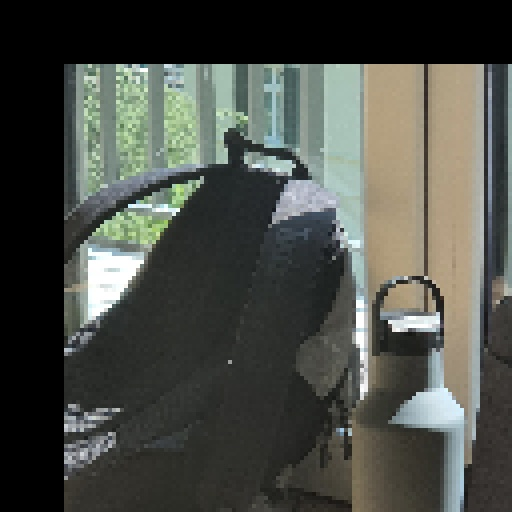
\includegraphics[width=0.19\textwidth]{img/correlation.jpg}}
    \subfigure[convolution]{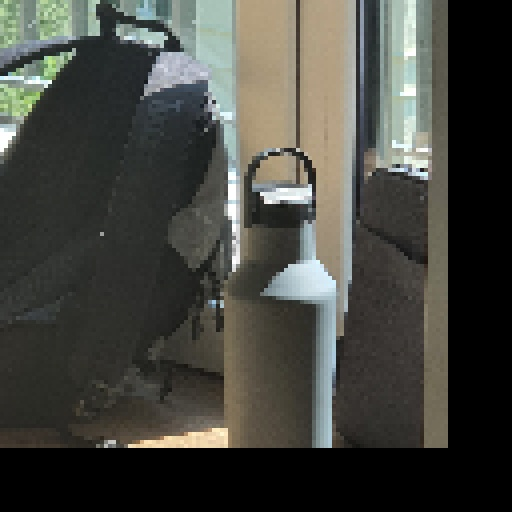
\includegraphics[width=0.19\textwidth]{img/convolved}}
    \caption{Difference between Correlation and Convolution Filtering by translating 32 pixels}
\end{figure}\end{minipage}

By rotating the kernel $180^\circ$, it is possible to get the same output from convolution filtering with correlational filtering and vice versa\cite{Gonzalez_Woods_2018}.

An apparent problem from neighborhood filtering is that on the edges, the neighbors simply does not exist in one or two directions 
(e.g. a $1000\times1000$ image passed through a $3\times3$ kernel would produce a $998\times998$ image). 
There are a couple method to alleviate the calculation of the nonexistent neighbors.

\subsection{Padding (Border Effects)}

\begin{minipage}{\textwidth}\begin{figure}[H]
    \centering
    \subfigure[zero]{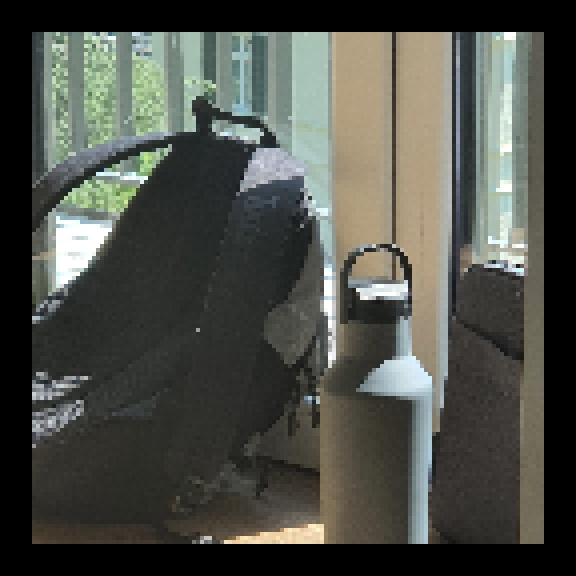
\includegraphics[width=0.19\textwidth]{img/border_constant}}
    \subfigure[wrap]{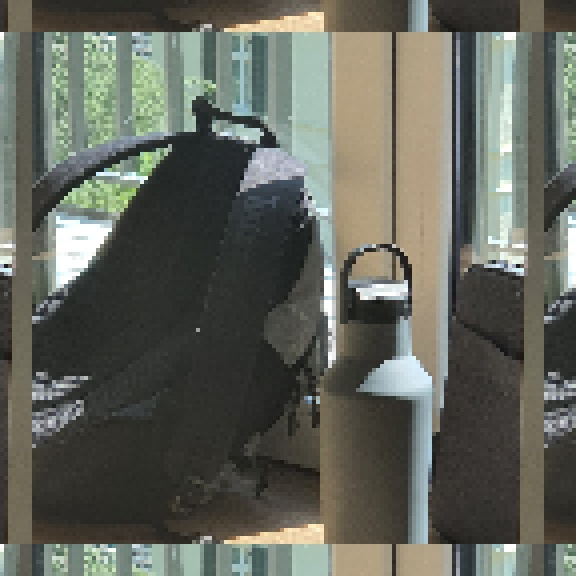
\includegraphics[width=0.19\textwidth]{img/border_wrap}}
    \subfigure[clamp]{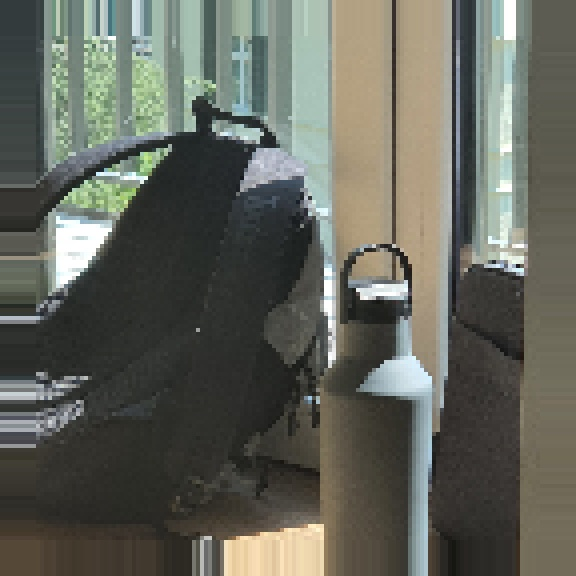
\includegraphics[width=0.19\textwidth]{img/border_clamp}}
    \subfigure[mirror]{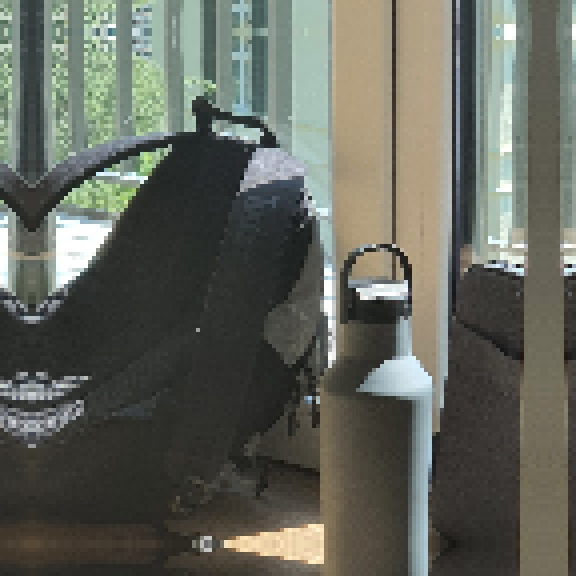
\includegraphics[width=0.19\textwidth]{img/border_reflect}}
    \subfigure[extend]{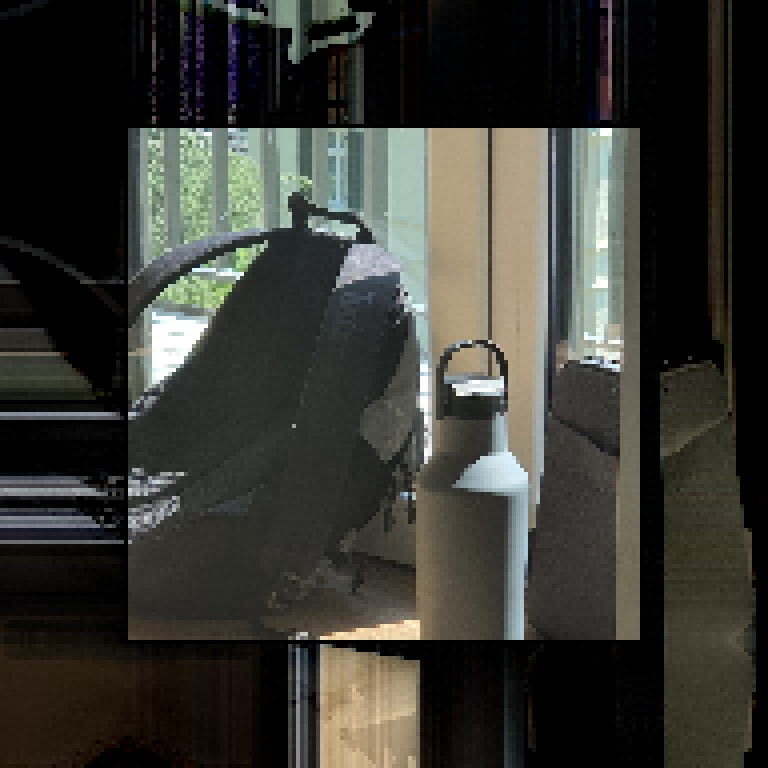
\includegraphics[width=0.19\textwidth]{img/border_extend.jpg}}
    \caption{Different types of border padding}
    \label{fig:padding_borders}
\end{figure}\end{minipage}
\begin{itemize}
    \item \textbf{Zero:} Set all pixels outside the region to zero.
    \item \textbf{Constant:} This is similar to Zero, but instead a specific color is chosen to replace the out of bound pixels.
    \item \textbf{Clamp:} The edge pixels are repeated indefinitely.
    \item \textbf{(Cyclic) Wrap (Repeat or Tile):} The entire image is repeated similar to tiling it infinitely.
    \item \textbf{Mirror:} The image is mirrored accordingly on each of the edges.
    \item \textbf{Extend:} This is a combination of clamping and mirroring, where the clamped image is subtracted with the mirrored image.
\end{itemize}\label{chap:padding}

This of course not only affects the unseen pixels, but the effects can bleed into the pixels inside the frame.
\begin{minipage}{\textwidth}\begin{figure}[H]
    \centering
    \subfigure[zero]{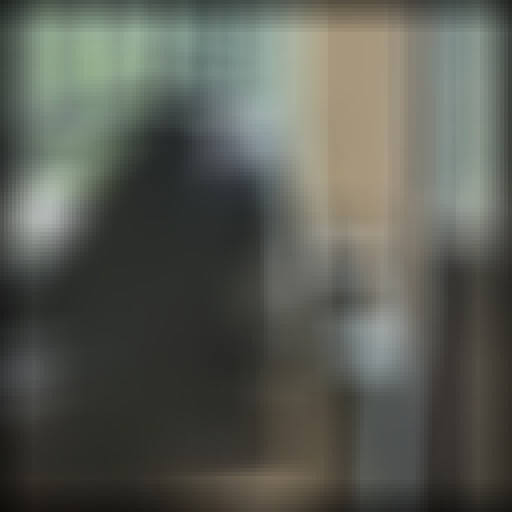
\includegraphics[width=0.19\textwidth]{img/boxBlur_constant}}
    \subfigure[wrap]{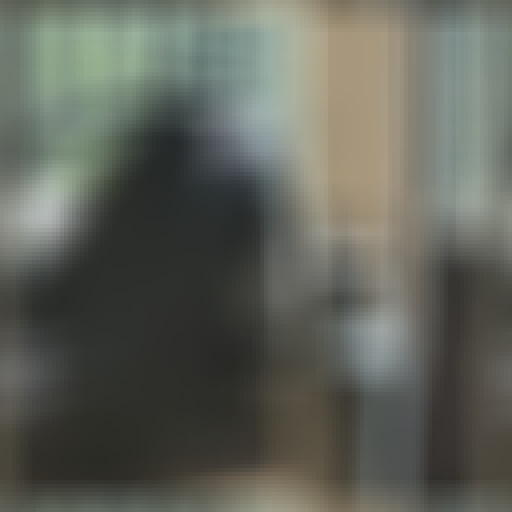
\includegraphics[width=0.19\textwidth]{img/boxBlur_wrap}}
    \subfigure[clamp]{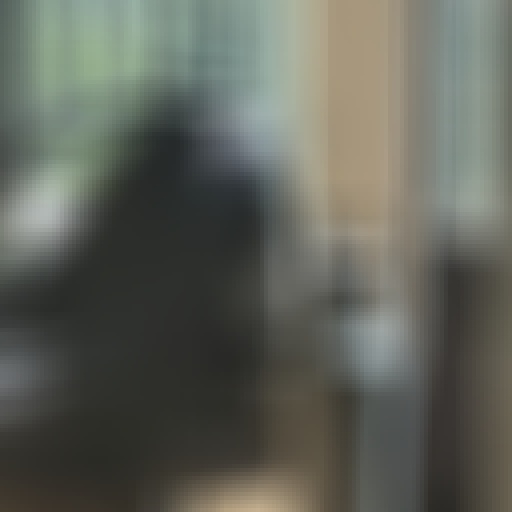
\includegraphics[width=0.19\textwidth]{img/boxBlur_clamp}}
    \subfigure[mirror]{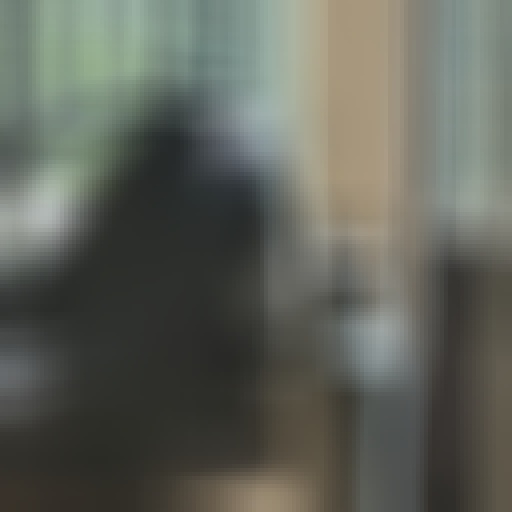
\includegraphics[width=0.19\textwidth]{img/boxBlur_reflect}}
    \subfigure[extend]{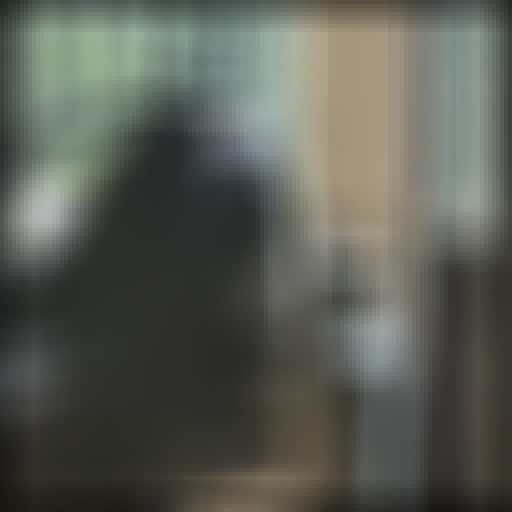
\includegraphics[width=0.19\textwidth]{img/boxBlur_extend.jpg}}
    \caption{Effects of different paddings with box blur}
    \label{fig:boxBlur_borders}
\end{figure}\end{minipage}

As seen from Figure \ref{fig:boxBlur_borders}, with a constant padding, the color chosen for the constant value bleeds uniformly in the edges. The wrapped image
can be convincing at times, but drastic changes from one border to another may lead to undesirable bleeding edges. If we instead clamp the image, the repeated pixels are noticeably
present, depending on the kernel size, this may still be desireable. In this use case, mirror seems to be the most convincing. It cannot however be said, that mirror is objectively the better
method, as it depends on the scenarios and use cases (e.g. if a subject is placed in a white background, then the constant padding may be desirable).

There are other ways to handle the borders such as two-phase duplication,
which is similar to clamp but alternates between the last 2 pixels.
A change in the filter function per individual basis can also be implemented, but it might not be practical,
as large amounts of additional logic may be needed\cite{BaileyAmbikumar18}.

\subsection{Separable Filtering}
The time complexity to calculate a single pixel can be said to be $O(M \cdot N)$ as it is dependent
on the size of the kernel. For each of the pixel in the kernel, it must be both multiplied and summed together
with its neighbors. This can be in practice sped up by separating the horizontal and vertical operations, hence performing
a one dimensional convolution horizontally, then one additional operation for the vertical convolution. This kernel in this case is the
outer product of two one dimensional kernels\cite{Szeliski_2022}. 
\[
    \boldsymbol{K} = v \otimes h = 
    \begin{bmatrix}
        v_1h_1 & v_1h_2 & v_1 h_3 & \hdots & v_1h_n \\
        v_2h_1 & v_2h_2 & v_2 h_3 & \hdots & v_2h_n \\
        \vdots & \vdots & \vdots & \ddots & \vdots \\
        v_m h_1 & v_m h_2 & v_m h_3 & \hdots & v_m h_n \\
    \end{bmatrix}
\]

Also notated as $K=vh^{\boldsymbol{T}}$, where $\boldsymbol{T}$ denotes transposing $h$, since both are supposedly vertical tuples.

A method to check whether a given Kernel is separable is to use \emph{Singular Value Decomposition (SVD)} \cite{Szeliski_2022}

\[        
    \boldsymbol{K} = \sum_{i}{\sigma_i \cdot u_i \cdot v_i^{\boldsymbol{T}}} 
\]
or more generally
\begin{align*}
        \boldsymbol{K} =& \textbf{U}_{m\times p} \boldsymbol{\textstyle\sum}_{p\times p} \textbf{V}_{p\times n}^{\boldsymbol{T}} \\
        \boldsymbol{K} =& \begin{bmatrix}
            u_0 & \hdots & u_{p-1}
        \end{bmatrix}
        \begin{bmatrix}
            \sigma_0&&\\
            &\ddots&\\
            &&\sigma_{p-1}
        \end{bmatrix}
        \begin{bmatrix}
            v_0 \\
            \vdots \\
            v_{p-1}
        \end{bmatrix}
\end{align*}
Note that it requires the number of rows and columns must be the same, it can however be solved by putting 0 as the missing rows/columns,
to allow the kernel to be a square matrix.Then the first singular value $\sigma_0$ is checked. If it is the only one that is non zero,
and the rest is zero, then the kernel is separable. As an example, the sobel filter, which is used for edge detection, 
can be separated into two separate operations. In this case, this is for the horizontal derivative approximation. \cite{CHANG2023160}
\[
    \frac{1}{8}
    \begin{bmatrix}
        -1 & 0 & 1 \\
        -2 & 0 & 2 \\
        -1 & 0 & 1
    \end{bmatrix}
    =
    \frac{1}{8}
    \begin{bmatrix} -1 & 0 & 1 \end{bmatrix}
    \begin{bmatrix} 1 \\ 2 \\ 1 \end{bmatrix}
\]
The normalization of the operators are easily calculated by dividing each operator with the absolute sum of the entries.
\[  
    \begin{bmatrix} -1 & 0 & 1 \end{bmatrix} \Rightarrow \vert -1 \vert + \vert 0 \vert + \vert 1 \vert = 2 \Rightarrow \frac{1}{2}
\]
Then the normalized operator is
\[
    \frac{1}{2} \begin{bmatrix} -1 & 0 & 1 \end{bmatrix}
\]
it applies to the vertical operator as well
\[
    \frac{1}{4} \begin{bmatrix} 1 \\ 2 \\ 1 \end{bmatrix}
\]
The following are more examples of common separable filtering.

\begin{center}\begin{tabular}{c c c c c}
    $
        \frac{1}{K^2}
        \begin{bmatrix}
           1 & 1 & \hdots & 1 \\
           1 & 1 & \hdots & 1 \\
           \vdots & \vdots & \ddots & \vdots \\
           1 & 1 & \hdots & 1
        \end{bmatrix}
    $
&
    $
        \frac{1}{16}
        \begin{bmatrix}
            1 & 2 & 1 \\
            2 & 4 & 2 \\
            1 & 2 & 1
        \end{bmatrix}
    $
& 
    $
        \frac{1}{256}
        \begin{bmatrix}
            1 & 4 & 6 & 4 & 1 \\
            4 & 16 & 24 & 16  & 4 \\
            6 & 24 & 36 & 24 & 6 \\
            4 & 16 & 24 & 16  & 4 \\
            1 & 4 & 6 & 4 & 1
        \end{bmatrix}
    $
& 
    $
        \frac{1}{8}
        \begin{bmatrix}
            -1 & 0 & 1 \\
            -2 & 0 & 2 \\
            -1 & 0 & 1
        \end{bmatrix}
    $
& 
    $
        \frac{1}{4}
        \begin{bmatrix}
            1 & -2 & 1 \\
            -2 & 4 & -2  \\
            1 & -2 & 1
        \end{bmatrix}
    $
\\
    $
        \frac{1}{K} 
        \begin{bmatrix} 1 & 1 & \hdots & 1 \end{bmatrix}
    $
&
    $
        \frac{1}{4} 
        \begin{bmatrix} 1 & 2 & 1 \end{bmatrix}
    $
&   
    $
        \frac{1}{16}
        \begin{bmatrix} 1 & 4 & 6 & 4 & 1 \end{bmatrix}
    $
&   
    $
        \frac{1}{2} 
        \begin{bmatrix} -1 & 0 & 1 \end{bmatrix}
    $
&
    $
        \frac{1}{2} 
        \begin{bmatrix} -1 & 2 & 1 \end{bmatrix}
    $
\\
Box & Bilinear & Gaussian & Sobel & Corner 
\end{tabular}\end{center}

Note that for Corner filtering, the kernel is not normalized. Normalization is important as otherwise, a pixel may go beyond the allowed value range.
In cases where the kernel has a negative value, it means that the pixel value is inverted, since an integer overflow occurs (e.g. $64
(-1)= -64 \mod 256 = 192$ for one channel in an 8 bit pixel).`'
With some filters, it is not always possible to separate it into just two operations, therefore it can be
transformed into a series of 1 dimensional operations. However, this may be impractical as it increases the time and space
complexity.

\subsection{Examples of Linear Filters}
Due to the fact that linear filter in essence is the sum of pixels in a neighborhood with varying weights and sizes, there are infinitely many different kernels that can
define operators which classified as linear and invariant. It is also even possible to factor in different color channels. As an example, it is possible to shift the hue of an image.
In this example, using a kernel of $\begin{bmatrix}0 & 0 & 1\end{bmatrix}$, the hue is shifted to the left (negative).
\lstset{language=Python}
\begin{lstlisting}
img = cv.imread("color.jpg")
kernel = np.array([[[0, 0, 1]]])
convolved = ndimage.convolve(img, kernel, mode='reflect')
cv.imwrite('../img/colorShift.jpg', convolved)
\end{lstlisting}


\begin{minipage}{\textwidth}\begin{figure}[H]
    \centering
    \subfigure[original]{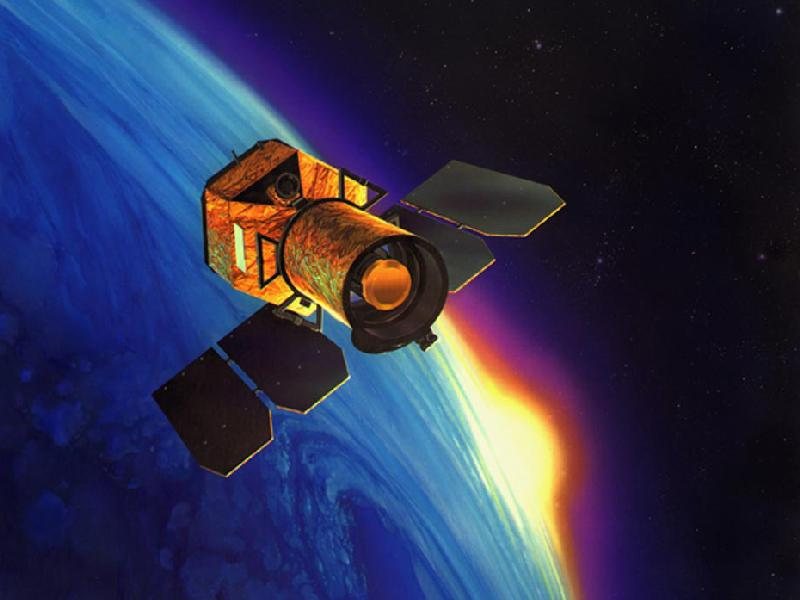
\includegraphics[width=0.30\textwidth]{codes/color.jpg}}
    \subfigure[shifted]{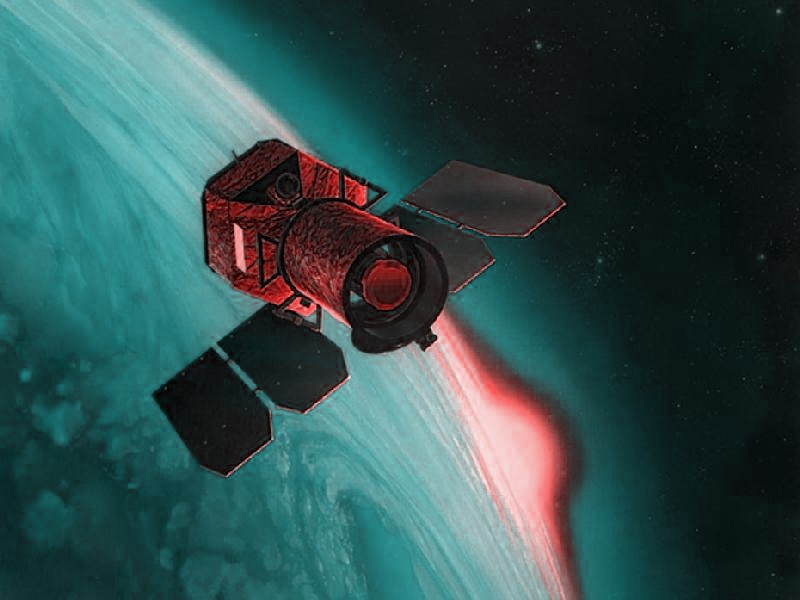
\includegraphics[width=0.30\textwidth]{img/colorShift.jpg}}
    \caption{Hue shifting using linear filters of the GALEX telescope image\cite{NASA_on_The_Commons_23}}
    \label{fig:hueshift}
\end{figure}\end{minipage}

The simplest application for linear filters are for smoothing(blurring) images. This not only serves their inherent purpose, but as later discussed, it can be used to aid other applications such as
edge detection or image enhancement.
\begin{itemize}
    \item \textbf{Box Filter:} each pixel is determined by the average of a $K \times K$ 
        neighborhood of pixels. It is also often called the \emph{moving average}, as the calculation can be done with scanlines, subtracting the
        old pixel and adding the newest pixels to the running sum. As the pixel is influenced equally by a square neighborhood, this may not be ideal as some `square artifacts' can be seen.
    \item \textbf{Bartlett Filter:} one solution to this is by separably convolving the image
        with a linear `tent' function (having its peak in the middle). A $3\times 3$ version of this is called the bilinear kernel.
    \item \textbf{Approximate Gaussian Filter:} if the Bartlett kernel is convolved with itself, this will produce an approximate version of the gaussian kernel.
\end{itemize}

This intuitively can be used to reduce the amount of noise on a picture. However, since it naively blurs the entire image,
details are also lost in the process.\\
\begin{minipage}{\textwidth}\begin{figure}[H]
    \centering
    \subfigure[original]{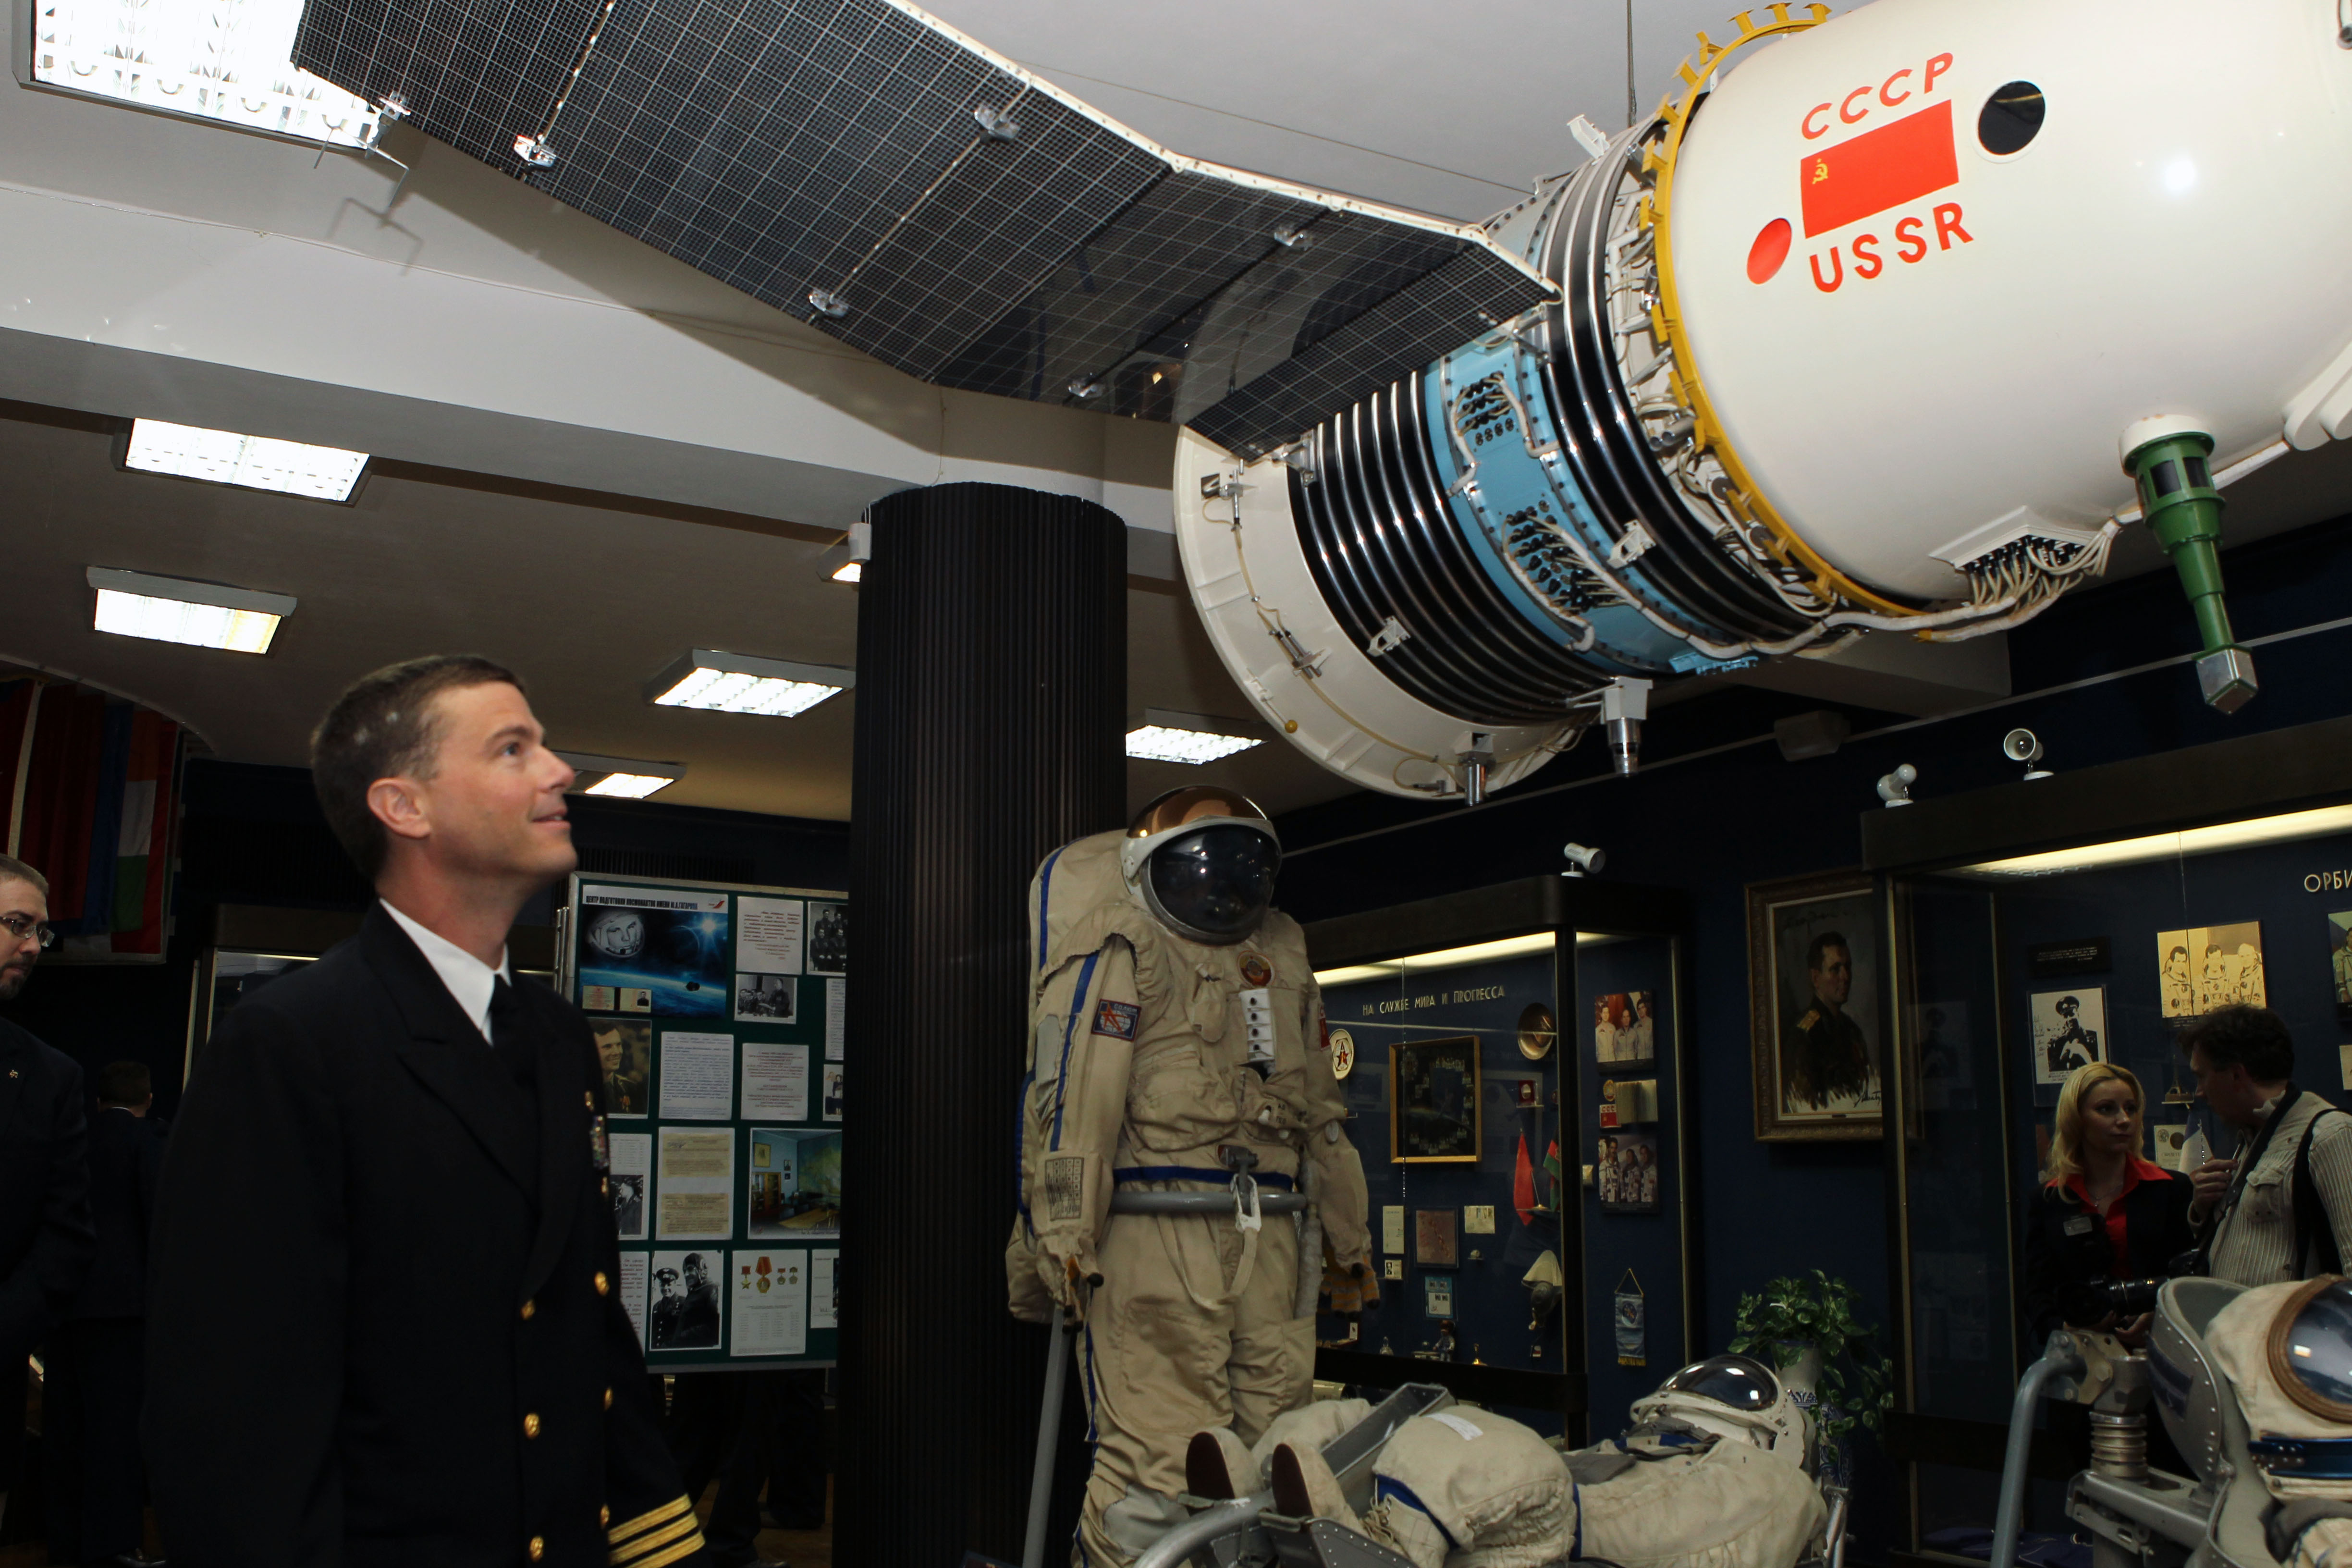
\includegraphics[width=0.32\textwidth]{codes/original_noise.jpg}}
    \subfigure[noise]{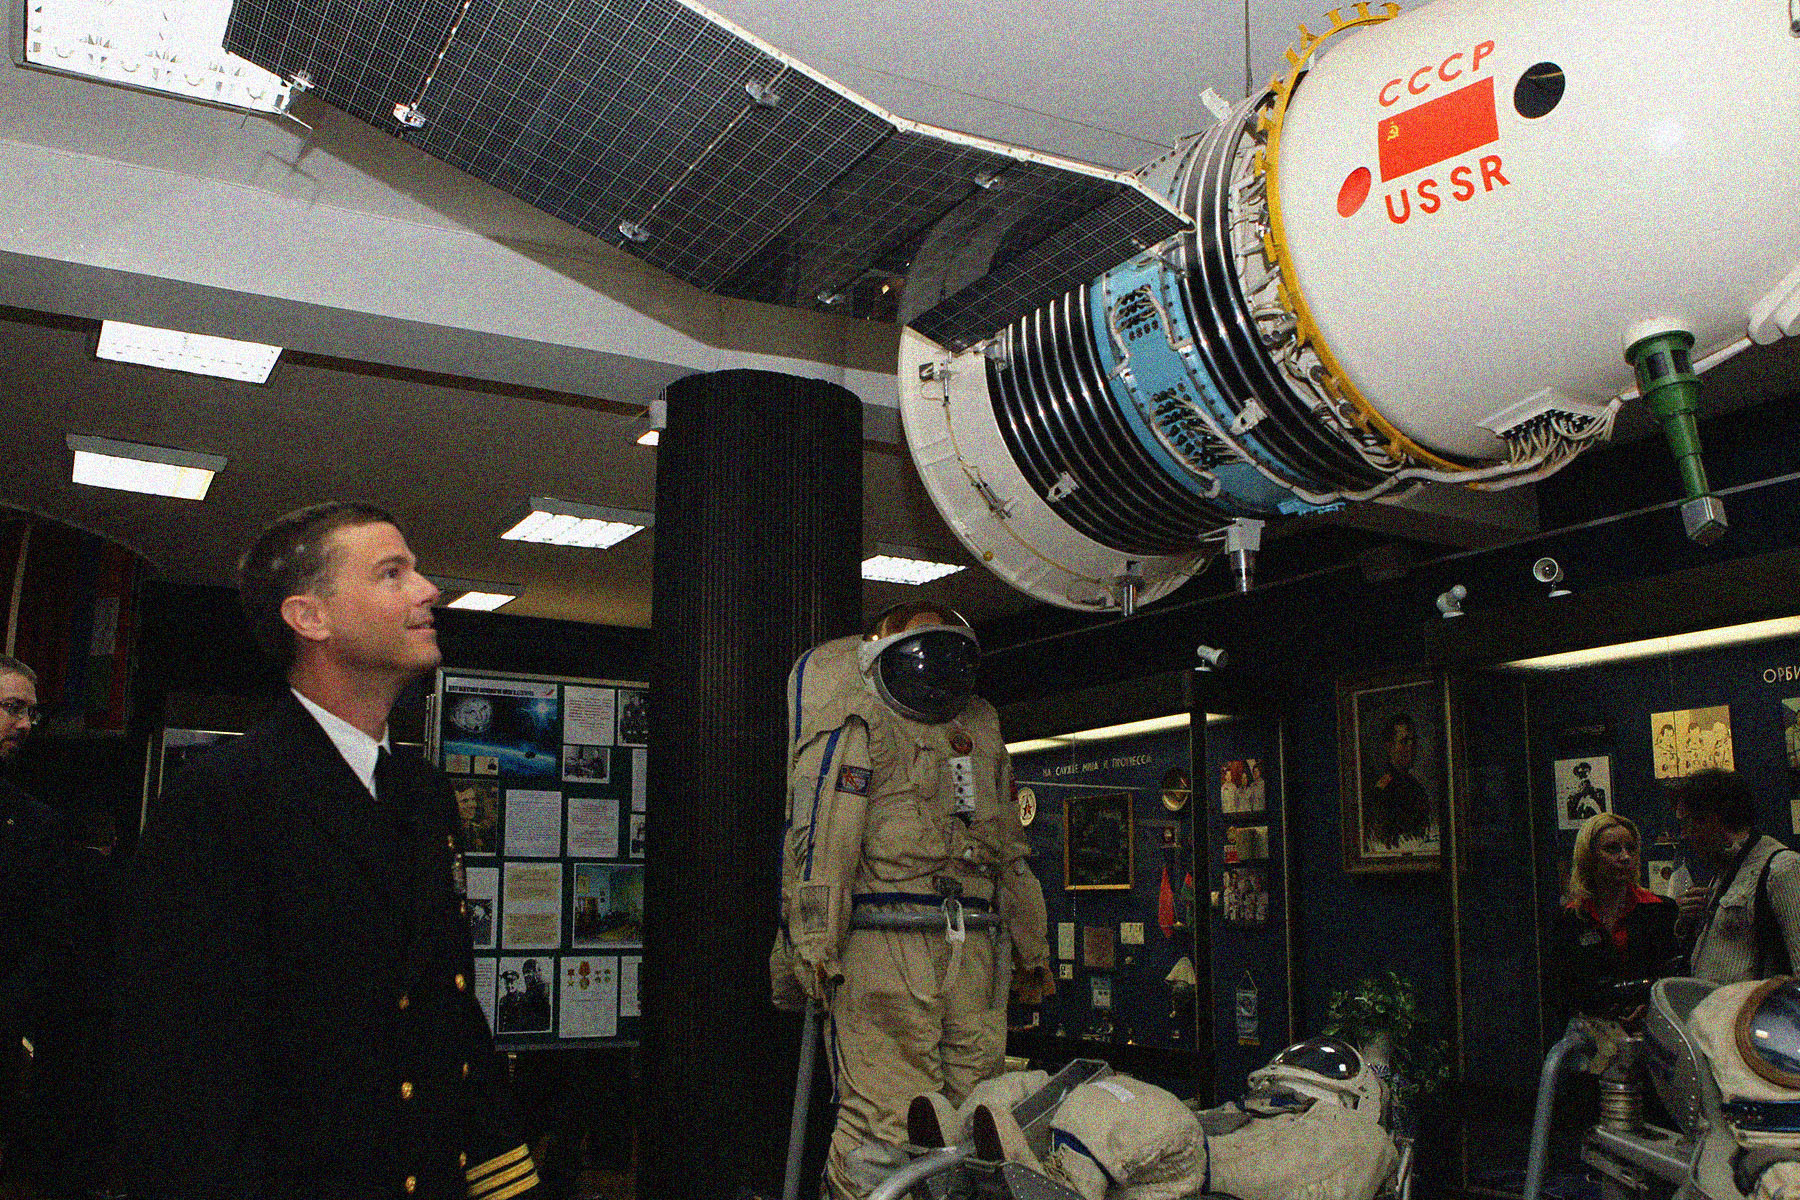
\includegraphics[width=0.32\textwidth]{codes/noise.jpg}}
    \subfigure[gaussian]{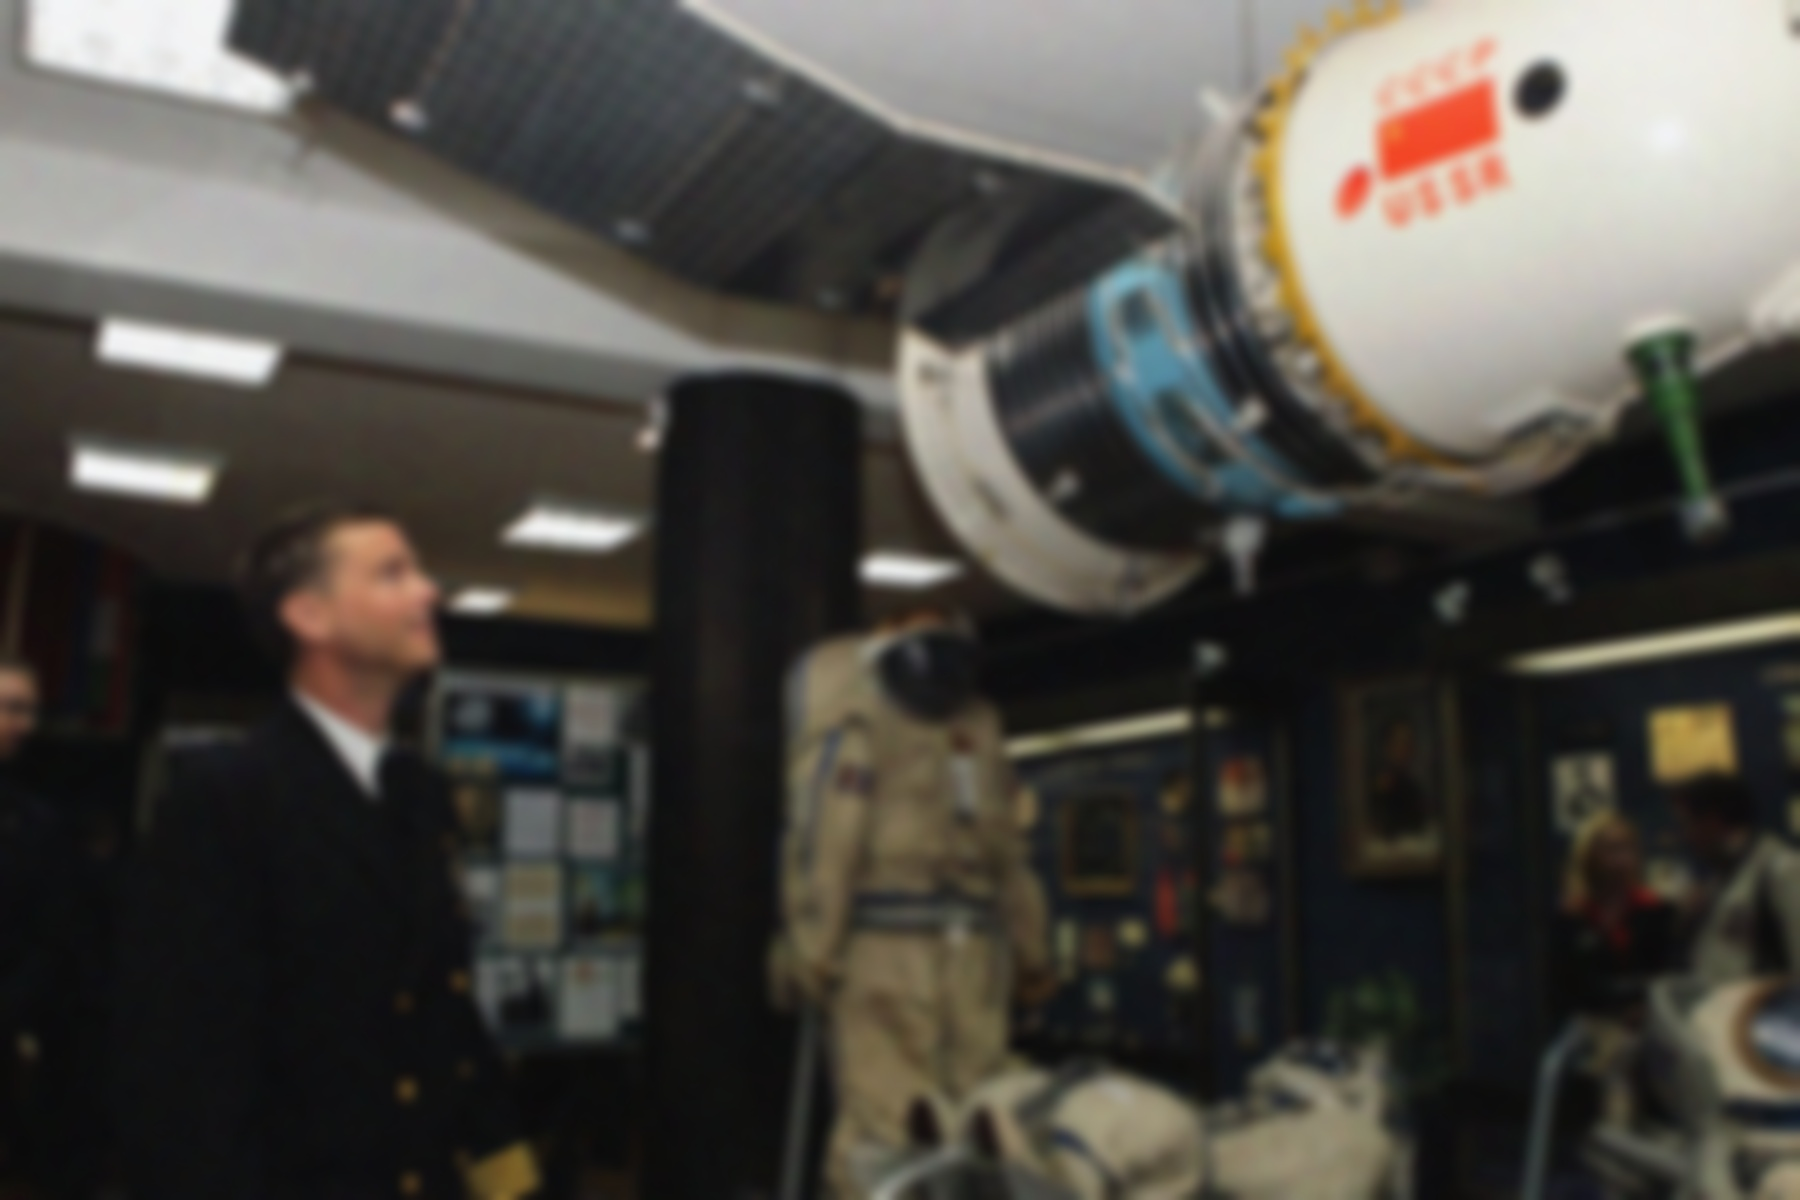
\includegraphics[width=0.32\textwidth]{img/noiseSuppressed.jpg}}
    \caption{(a) Original image of the Star City Museum\cite{NASA_on_The_Commons_14}(b) Noise added artificially (c) Blurred with Gaussian (k=27 $\sigma=7$)}
    \label{fig:noise}
\end{figure}\end{minipage}

Essentially, the three above filters are different mathematical functions applied both horizontally and vertically.\\
\begin{minipage}{\textwidth}\begin{figure}[H]
    \centering
    \subfigure[Average]{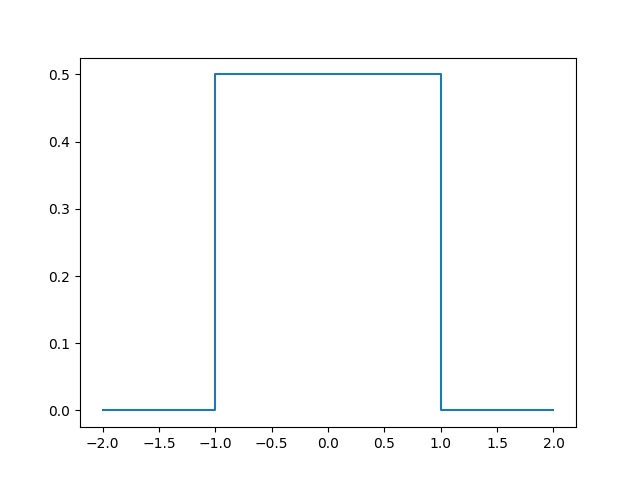
\includegraphics[width=0.29\textwidth]{img/box_graph.png}}
    \subfigure[Bartlett (Tent)]{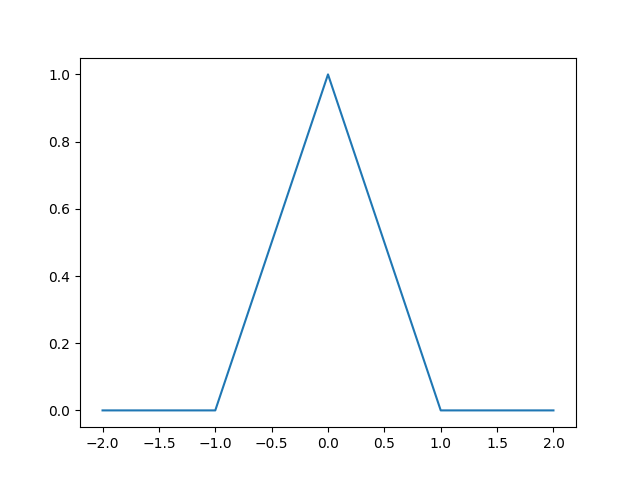
\includegraphics[width=0.29\textwidth]{img/tent_graph.png}}
    \subfigure[Gaussian]{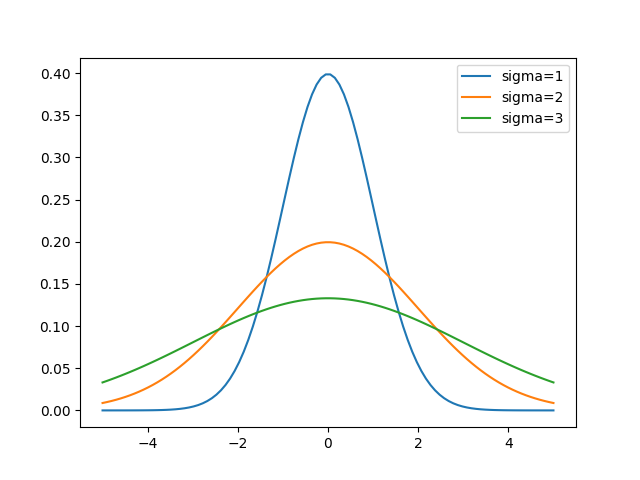
\includegraphics[width=0.29\textwidth]{img/gaussian_graph.png}}
    \caption{One dimensional graphs of the filters}
    \label{fig:graph}
\end{figure}\end{minipage}
As its name suggests, the Gaussian Filter is based on the Gaussian function (also commonly known as the normal function).
Two dimensionally, it can be expressed as \cite{MISRA2020289}
\[
    G_{2D}(x, y, \sigma) = \frac{1}{2\pi\sigma^2}e^{-\frac{x^2 + y^2}{2\sigma^2}}
\]
It can be seen from the graph that the lower the sigma value, the narrower the neighborhood becomes. 


\begin{minipage}{\textwidth}\begin{figure}[H]
    \centering
    \subfigure[Box $(k=133)$]{
\includegraphics[width=0.29\textwidth]{img/blurBox.png}}
    \subfigure[Gaussian $(k=233)$]{
\includegraphics[width=0.29\textwidth]{img/blurGaussian.png}}
    \caption{Comparison between gaussian and box blur}\label{fig:gauss_box}
\end{figure}\end{minipage}
From Figure \ref{fig:gauss_box}, using the gaussian blur, as opposed to
the box filter produces a more appealing image, as it preserves the shape of the image better as opposed to creating this `halo' effect
and producing a squashed rectangular shape in the center. One disadvantage to Gaussian however is, to produce an equally `blurred' image, a larger kernel is required for Gaussian, which can be argued to then be slower
than using the box filter\cite{Gonzalez_Woods_2018}.


These filters are mainly used to smoothen(blur) the image, where the low frequencies are let through as well as reducing the effect of the high frequencies (high frequencies and low frequencies both referring to
the brightness/darkness of each pixel). In practical applications, this is done to reduce high frequency noises.
A creative application to smoothing the images, is that the smoothen images can be used as a mask to sharpen the image by adding the difference between the original and blurred image.
This method is called \emph{unsharp masking}, aiming to enhance the difference between the shadows and higlights on an image\cite{Szeliski_2022}.
\[
  g_{sharp} = f + \gamma(f - h_{blur} \ast f)  
\]
\begin{minipage}{\textwidth}\begin{figure}[H]
    \centering
    \subfigure[original]{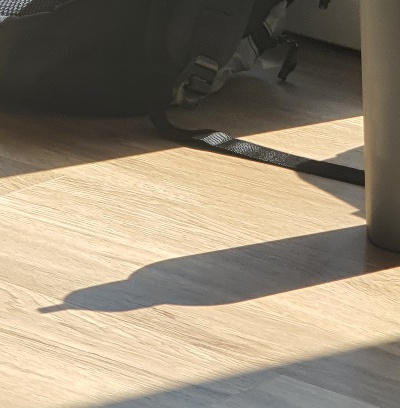
\includegraphics[width=0.19\textwidth]{img/original_mask.jpg}}
    \subfigure[unsharp mask]{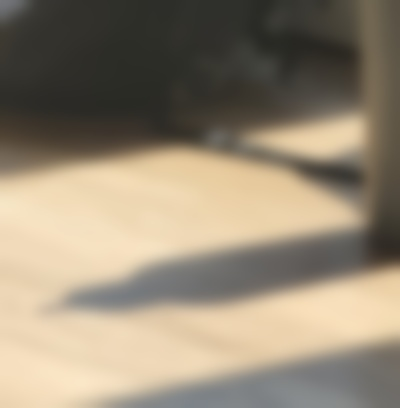
\includegraphics[width=0.19\textwidth]{img/unsharp_mask.jpg}}
    \subfigure[difference]{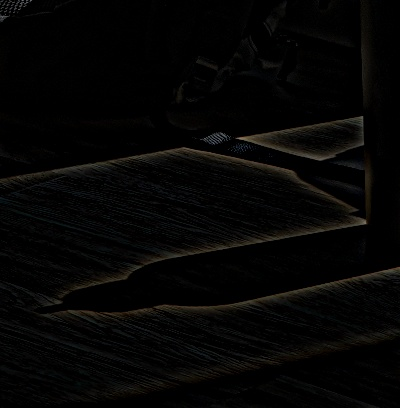
\includegraphics[width=0.19\textwidth]{img/difference_unsharp.jpg}}
    \subfigure[sharpened]{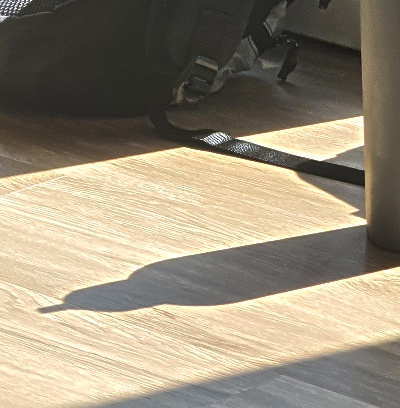
\includegraphics[width=0.19\textwidth]{img/sharpened.jpg}}
    \caption{Unsharp masking with Gaussian blur}\label{fig:unsharp_mask}
\end{figure}\end{minipage}
The result of the image traces a bright outline througout the image between the darker(shadow) and lighter part. It can also be seen, that
the difference between the blurred image and the original results in an approximate edge detection. A better way to extract edges by means of linear filtering is
by the use of the \emph{Sobel filter}. \cite{Szeliski_2022}

\subsection{Sobel Filter}
As per the example in the previous section, the horizontal Sobel operator is calculated by combining the \emph{horizontal central difference}
(which calculates the second horizontal derivative of the pixel and places it in the center itself) and a vertical linear tent filter to smooth the result. Respectively, it can also
be done for the vertical derivative.

The two sobel operator emphasizes the horizontal or vertical edges respectively, although as seen in the images, it can also highlight diagonal edges.\\
\begin{minipage}{\textwidth}\begin{figure}[H]
    \centering
    \subfigure[original]{\includegraphics*[width=0.29\textwidth]{codes/nasa.jpg}}
    \subfigure[horizontal]{\includegraphics[width=0.29\textwidth]{img/sobelHorizontal.png}}
    \subfigure[vertical]{\includegraphics[width=0.29\textwidth]{img/sobelVertical.png}}
    \caption{Vertical and Horizontal Sobel filtering\cite{NASA_on_The_Commons_2023}}\label{fig:sobel}
\end{figure}\end{minipage}

\subsection{Band-pass and steerable Filter}
In the above example, the sobel filter is calculated either for the horizontal or
vertical axis. Nevertheless, it is possible to calculate filters (including for sobel) for any angles in between using a specified 
\emph{directional derivative} $\nabla_{\boldsymbol{\hat{u}}} = \frac{\partial}{\partial\boldsymbol{\hat{u}}}$ 
and a \emph{unit direction} $\boldsymbol{\hat{u}} = (\cos \theta, \sin \theta)$\cite{Szeliski_2022}.
\[
    \boldsymbol{\hat{u}} \cdot \nabla (G \ast f) = \nabla_{\boldsymbol{\hat{u}}}(G \ast f) = (\nabla_{\boldsymbol{\hat{u}}}G) \ast  f
\]
Then it is also preferable to smooth it with the Gaussian filter.
\[
    G_{\boldsymbol{\hat{u}}} = u G_x + v G_y = u \frac{\partial G}{\partial x} + v \frac{\partial G}{\partial y} 
\]
This is called the \emph{directional} or \emph{oriented} filter.

A similar to operator to the sobel filter is called the \emph{Prewitt operator}, which instead of convolving it with a perpendicular tent filter,
it instead uses an average operator. Commonly however, the Sobel operator is preferred as it provides better performance\cite{NIXON2020141}. Through testing, the Sobel Operator seems
to be less selective than the Prewitt Operator, but one can argue that the Prewitt is then preferred as it is more accurate.

\begin{minipage}{\textwidth}\begin{figure}[H]
    \centering
    \subfigure[Pattern]{\includegraphics*[width=0.29\textwidth]{codes/pattern.png}}
    \subfigure[Sobel]{
\includegraphics[width=0.29\textwidth]{img/directionSobel.png}}
    \subfigure[Prewitt]{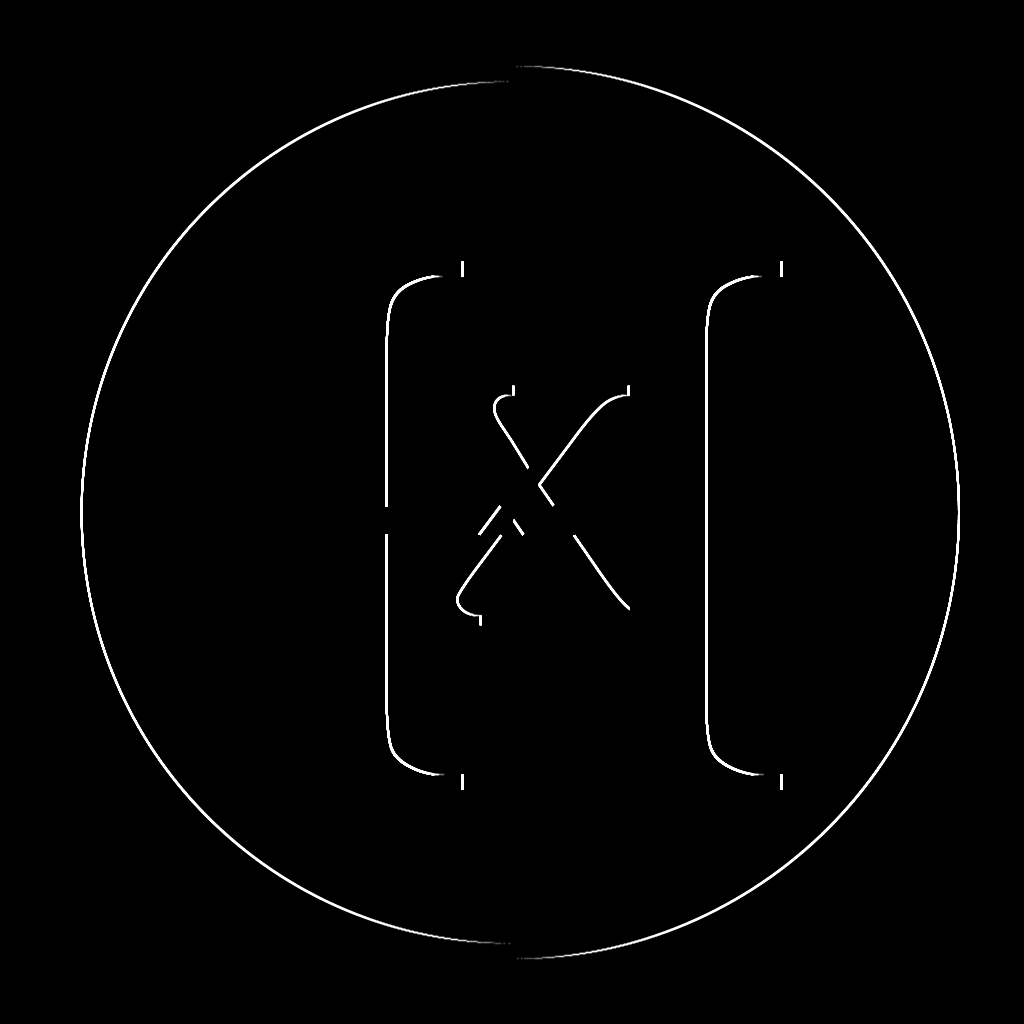
\includegraphics[width=0.29\textwidth]{img/directionScharr.png}}
    \caption{Vertical edge detection using Sobel and Prewitt on a test pattern}\label{fig:pattern}
\end{figure}\end{minipage}

As seen on Figure \ref{fig:pattern}, the Sobel filter tapers the edges at the top into a gradient, whereas the Prewitt marks it confidently without tapering. In practice however,
the minimal difference might not be worth the difference in the additional compute time \cite{NIXON2020141}.

\begin{minipage}{\textwidth}\begin{figure}[H]
    \centering
    \subfigure[]{
        {$\begin{bmatrix}
            -1 & 0 & 1 \\
            -2 & 0 & 2 \\
            -1 & 0 & 1
        \end{bmatrix}$}
    }
    \subfigure[]{
        {$\begin{bmatrix}
            1 & 0 & -1 \\
            1 & 0 & -1 \\
            1 & 0 & -1
        \end{bmatrix}$}
    }
    \subfigure[]{
        {$\begin{bmatrix}
            1 & 1 & 1 \\
            0 & 0 & 0 \\
            -1 & -1 & -1
        \end{bmatrix}$}
    }
    \caption{Sobel and Prewitt operator comparison (a) Horizontal Sobel operator; 
    (b) Horizontal Prewitt operator; (c) Vertical Prewitt operator}\label{fig:prewittSobel}
\end{figure}\end{minipage}


Another filter is called the \emph{Laplacian operator}, which is the second (undirected)derivative.\cite{Szeliski_2022}
\[
    \nabla^2 f = \frac{\partial^2 f}{\partial x^2} + \frac{\partial^2 f}{\partial y^2}
\]
and again, it can be smoothed with the Gaussian filter. It is equivalent to the \emph{Laplacian of Gaussian}(LoG) filter.
\[
    \nabla^2 G (x, y, \sigma) = (\frac{x^2 + y^2}{\sigma^4} - \frac{2}{\sigma^2}) G (x, y, \sigma)
\]
\begin{minipage}{\textwidth}\begin{figure}[H]
    \centering
    \subfigure[]{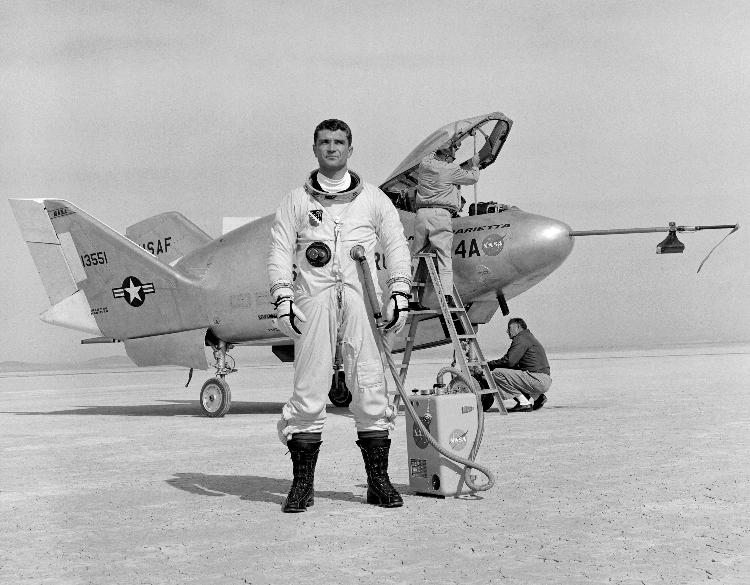
\includegraphics[width=0.29\textwidth]{img/laplacianOriginal.png}}
    \subfigure[]{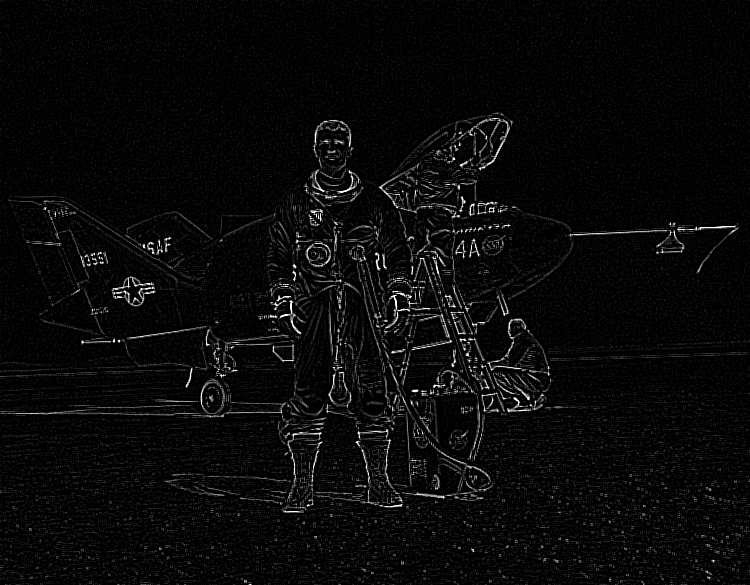
\includegraphics[width=0.29\textwidth]{img/laplacian.png}}
    \subfigure[]{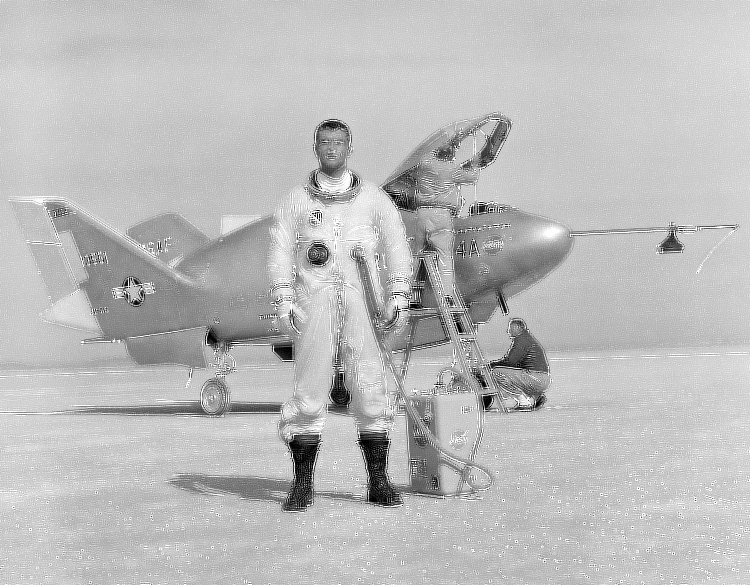
\includegraphics[width=0.29\textwidth]{img/laplacianAdded.png}}
    \caption{Laplacian Filtering (a) Original image of NASA pilot\cite{NASA_on_The_Commons_1970}; (b) Output of the laplacian filter with Gaussian blur (c) Combined image of the orientation map and original}
    \label{fig:padding_borders}
\end{figure}\end{minipage}

Since the laplacian filter does not rely on a specific direction, it can be seen at the above picture that the edges are agnostic to the direction and not biased to a certain angle. Bear in mind that smoothing the picture (in this case by means of the Gaussian filter)
is necessary as it subdues the noises from being detected as edges.

The aforementioned filters are more sophisticated as they require the second or first derivatives and they can filter both the low and high frequencies. 
These filters are called \emph{band-pass filters}.
Since the filters are based on the gradient fields, which are undirected, it can be `steered' by freely choosing a unit direction, hence the name
\emph{steerable} filter. The advantage of this is that multiple variations of directions can easily be calculated with minimal cost as the derivative must only be calculated once. In case of higher order derivatives,
the calculation must be done repeatedly with the same unit vector. This can although be calculated with a relatively small number of functions\cite{Szeliski_2022}. Consider the example below for the second-order derivatives,
which requires 3 basis functions. Although the basis filters are not in itself separable, it can be expressed as a linear combination of multiple separable filters.
\[
    G_{\boldsymbol{\hat{u}}\boldsymbol{\hat{u}}} = u^2 G_{xx} + 2uvG_{xy} + v^2 G_{yy} \text{with} \hspace*{0.5em}\boldsymbol{\hat{u}} = (u, v)
\]

With higher order steerable filters, it is possible to create filters that is more selective with the orientation (unlike in Figure \ref{fig:sobel}, where the lines placed at an angle of $45^\circ$ is highlighted). Alternatively,
it can also be possible to create filters that responds to more than one type of edge, whether bar edges (thin lines) or step edges (stark transitions between dark and light pixels), this however requires the \emph{Hilbert transform pairs}
\cite{Szeliski_2022}.

\begin{minipage}{\textwidth}\begin{figure}[H]
    \centering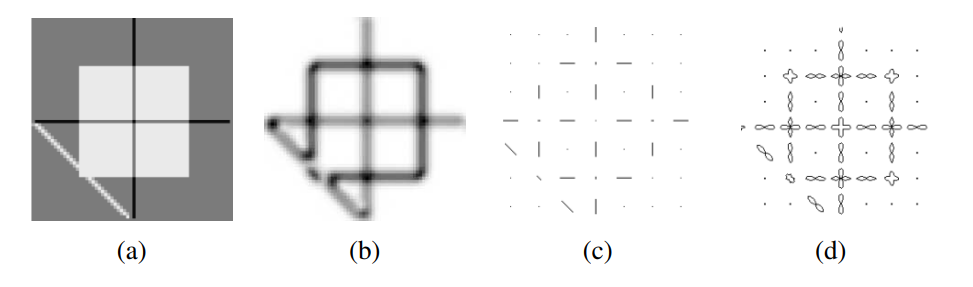
\includegraphics[width=0.60\textwidth]{img/higher.PNG}
    \caption{Fourth-order steerable filter (a) original test pattern (b) average oriented output (c) dominant orientation (d) oriented energy as a function of angle (polar plot)}\cite{Szeliski_2022}
\end{figure}\end{minipage}

Steerable filtering are most commonly used for edge detection, but another common use case is \emph{corner detection}. This requires multiple steerable operators in different directions as corners are defined as
points with a sharp change in direction (high curvature)\cite{NIXON2020141}. Feature description is also one application of steerable filter\cite{Szeliski_2022}.

\subsection{Summed area table (integral image)}
To calculate pixels in a neighborhood, some pixels needs to be accessed multiple times and as the kernel size increases, this problem also magnifies as well. To
better process the convolution of multiple box filters of different sizes and locations, preprocessing it can practically reduce the time complexity. 
This can be done with the
\emph{summed area table}, or the running sum of all the pixel values from the origin. It can be computed recursively through the raster-scan algorithm.
\[
    s(i, j) = s(i - 1, j) + s(i, j - 1) - s(i - 1,j - 1) + f(i, j)   
\]
This is also an example of recursive filtering, which takes a previous calculated value of a pixel and calculate it further for the next pixel. In this case, this can theoretically go on forever, but since no picture is infinite,
the edges can be calculated using the padding strategies in Section\ref{chap:padding}.

Since the calculations are based on previously calculated pixels, this attempts to reduce the amount of times a pixel is used for calculations, as it immediately takes the already calculated value
instead. The image $s(i, j)$, often called \emph{Integral image} can be computed using two additions per pixel. The summed area inside a chosen rectangl can be calculated by sampling 4 pixels from the summed area table.
\[
    S(i_0\hdots i_1, j_0\hdots j_1) = s(i_1, j_1) - s(i_1, j_0 - 1) - s(i_0 - 1, j_1) + s(i_0 - 1, j_0 - 1)
\]
 
\begin{minipage}{\textwidth}\begin{figure}[H]
    \centering
    \subfigure[Original image(S = 24)]{
        $\begin{tabular}{|c|c|c|c|c|}
            \hline 3 & 2 & 7 & 2 & 3 \\
            \hline 1 & \cellcolor{green!25}5 & \cellcolor{green!25}1 & \cellcolor{green!25}3 & 4 \\
            \hline 5 & \cellcolor{green!25}1 & \cellcolor{green!25}\textbf{3} & \cellcolor{green!25}5 & 1 \\
            \hline 4 & \cellcolor{green!25}3 & \cellcolor{green!25}2 & \cellcolor{green!25}1 & 6 \\
            \hline 2 & 4 & 1 & 4 & 8 \\
            \hline
        \end{tabular}$
    }
    \subfigure[Summed area table(S = 28)]{
        $\begin{tabular}{|c|c|c|c|c|}
            \hline 3 & 5 & 12 & 14 & 17 \\
            \hline 4 & \cellcolor{cyan!25}\textit{11} & \cellcolor{cyan!25}\textbf{19} & 24 & 31 \\
            \hline 9 & \cellcolor{cyan!25}\textbf{17} & \cellcolor{red!25}28 & 38 & 46    \\
            \hline 13 & 24 & 37 & 48 & 62 \\
            \hline 15 & 30 & 44 & 59 & 81 \\
            \hline
        \end{tabular}$
    }
    \subfigure[Computation of area sum (S = 24)]{
        $\begin{tabular}{|c|c|c|c|c|}
            \hline \cellcolor{blue!25}\textbf{3} & 5 & 12 & \cellcolor{blue!25}\textit{14} & 17 \\
            \hline 4 & \cellcolor{green!25}11 & \cellcolor{green!25}19 & \cellcolor{green!25}24 & 31 \\
            \hline 9 & \cellcolor{green!25}17 & \cellcolor{green!25}28 & \cellcolor{green!25}38 & 46 \\
            \hline \cellcolor{blue!25}\textit{13} & \cellcolor{green!25}24 & \cellcolor{green!25}37 & \cellcolor{blue!25}\textbf{48} & 62 \\
            \hline 15 & 30 & 44 & 59 & 81 \\
            \hline
        \end{tabular}$
    }
    \caption{Summed area tables\cite{Szeliski_2022}}
    \label{fig:graph}
\end{figure}\end{minipage}
The above table shows the relation of how the area is calculated. For summed area table, the red pixel is calculated by adding itself to the
two highlighted pixels in bold while subtracting the italicised symbol After the entire summed area table is calculated, it is now
cost effective to calculate the area sum as the sum of the top left and bottom right numbers only needs to be subtracted with the other diagonal (remember that
the starting indices requires it to go one pixel beyond the corresponding rectangle).

Although with this preprocessing it reduces the time complexity, the space complexity increases, since each pixel's range has now increased due to summing multiple pixel into a single pixel,
hence each of them now requires $\log M + \log N$ additional bits ($M$ and $N$ being the width and height)\cite{Szeliski_2022}.

A common use case for summed area table is for feature detections, computing simple multi-scale low-level features. In practice, it may be preferrable to instead use 
moving average filters, for example in computing the sum in the sum of squared differences stereo (SSD) and motion algorithms\cite{Szeliski_2022}.\footnotemark\footnotetext{Entire section of linear filtering is written by Jose}

% =========================================================================
\bibliographystyle{alpha}
\bibliography{abbrev, Draft}
\end{document}
